\chapter{Background}
\todo{Add some text here}
\section{Cross-site scripting}
\textit{Cross-site scripting} (or \textit{XSS} for short) is a special type of code injection attack in the Web. In XSS, the attacker tries to inject arbitrary (and probably harmful) JavaScript code into web pages that will eventually be displayed on one victim browser\footnotemark . Once the targeted browser receives the web page, it will execute all its contained JavaScript code including the injected malicious payload which, of course, has exactly the same privileges as any other legitimate JavaScript code exists in that page.

\begin{figure}
	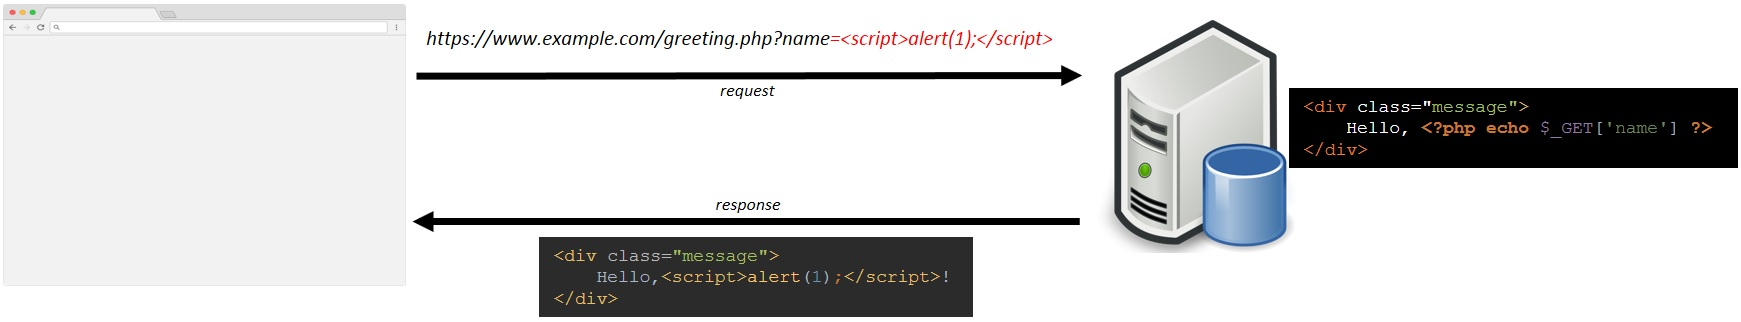
\includegraphics[width=\linewidth]{figures/xss_example.jpg}
	\caption{An example of reflected XSS attack}
	\label{fig:xss_example}
\end{figure}

Usually, XSS attack occurs as a result of exploiting a code injection vulnerability that persists in the target web application. In figure \ref{fig:xss_example}\todo{enlarge font in figure}, a PHP code snippet is responsible for displaying a small greeting message for the user. The value of the name is shipped within the name GET parameter and is included as part of the request URL. One attacker can induce the victim user to call an attacker-crafted request URL with the malicious payload being set to the name parameter. Without any string escaping mechanism or input filtering of the name value, the web application will simply inject that payload into the \verb!$_GET[‘name’]! placeholder once it receives the request and send the resultant HTML page back to the victim browser, which will in turn detect the injected script tag and executes its content resulting in XSS attack.

\footnotetext{Two types of XSS script injection mechanisms exist, namely Stored XSS and Reflected XSS. However, since injection techniques are out of the scope of this study, we omitted them from the discussion}

\section{XSS mitigations}
If we looked back at the vulnerable back-end code in figure \ref{fig:xss_example}, one can simply propose a code fix by which we filter out the input for any \verb|<script>| tag before it’s injected in the page. This filtering functionality will then be part of the web application logic. In real-world web applications, the web security community proposed a lot of secure code practices and standards to avoid such vulnerabilities (auto escaping templating systems, reporters and scanners)\footnotemark\todo{Need to add footnote text}. Nevertheless, at large scale, the process of detecting and fixing code injection bugs become a tedious task. Moreover, It was proven (cite) that it’s extremely difficult, at a large scale, to have a 100\% injection-bug-free web apps. Here is where XSS mitigations come into play. XSS mitigations share a very fundamental assumption; “XSS mitigations focus on preventing the attack instead of fixing the vulnerability”. So instead of looking for bugs, it tries to stop the attack itself, thus the application remains secure regardless of vulnerabilities existence. 

In our study, we consider four types of those mitigations:

\paragraph{Web application firewall WAFs} WAFs are placed in the server side, and provide filtering mechanism in which they look at all web traffic that come to the server and then apply a bunch of rules or regular expressions onto these requests in order to find potentially-malicious injected payloads. 
One well-known WAF that is heavily adopted in practice is ModSecurity  which is usually shipped with OWASP Core Rule Set (CRS); \todo{Need to be more specific here} a default set of detection and prevention rules for a wide range of XSS attack vector. 

\paragraph{Browser-based XSS filters} These mitigations work on the user-side and are deployed as and additional browser Add-on or as part of the browser default configuration. The first version of These filters do quite similar job as the WAF in which they monitor all HTTP requests that are leaving the browser looking for any maliciously-looking content and remove it (or block the entire request). One remarkable example of such filters is the Firefox NoScirpt add-on\todo{need a footnote}. Other variants\todo{We may use word "mode" here} of XSS filters we may encounter in practice are implemented by IE and Chrome XSS filters. This variant of XSS filter is slightly different from the one defined by NoScirpt in that; instead of only filtering the HTTP request looking for injected payloads, it also wait for the response from the server, and before the browser executes the response they look for malicious markup that was already detected in the request if it exists also in the response. If that was the case, they try to either remove the malicious payload from the response or block the whole requests.

\paragraph{Content Security Policy CSP} Recently A new XSS mitigation scheme. It tries to detect legitimate markup that is supposed to be in the page from illegitimate markup based on different mode, hence it allows the browser to execute legitimate code while preventing it from executing non-legitimate one. It has different ways of telling which is legitimate and which is malicous: 

\begin{itemize}
	\item Whitelising mode: In this mode, a finite set of valid web sources\todo{Add footnote} is defined and a script is considered legitimate when it comes from one of these sources only.
	\item Nonce-based mode: a script is considered legitimate if it was annotated with a correct secret cryptographic nonce.
\end{itemize}

\paragraph{Response Sanitizers} Sometimes you are in a situation where you have a user-provided string and you want to render it as an HTML. It may happen that, you want the user to be able to render some parts of the fonts to be italic and bold so you allow HTLM injection but you don’t want to allow malicious HTML injection. Sanitizers basically takes the string and remove all malicious parts out of it. So the assumption is that you have a safe string that you can render without XSS. They are JS libraries like DOMPurify and Chrome clouser. is that you have a safe string that you can render without XSS. They are JS libraries like DOMPurify and Chrome clouser.

